\paragraph{交织器的原理及作用}

在通信中,传输信息比特差错经常是成串发生的。然而,信道编码仅在检测和校正单个差错和不太长的差错串时才有效。为了解决这一问题,希望能找到把一条消息中的相继比特分散开的方法,即一条消息中的相继比特以非相继方式被发送。这样,在传输过程中即使发生了成串差错,恢复成一条相继比特串的消息时,差错也就变成单个(或长度很短),这时再用信道编码纠错功能纠正差错,恢复原消息。简单来说,交织就是将信道传输过程中的连续差错分散化。

\paragraph{交织器的实现}

本实验中采用最常见的交织方法——行列交织。行列交织基本的原理如下图所示:

\begin{figure}[htd]
    \centering
    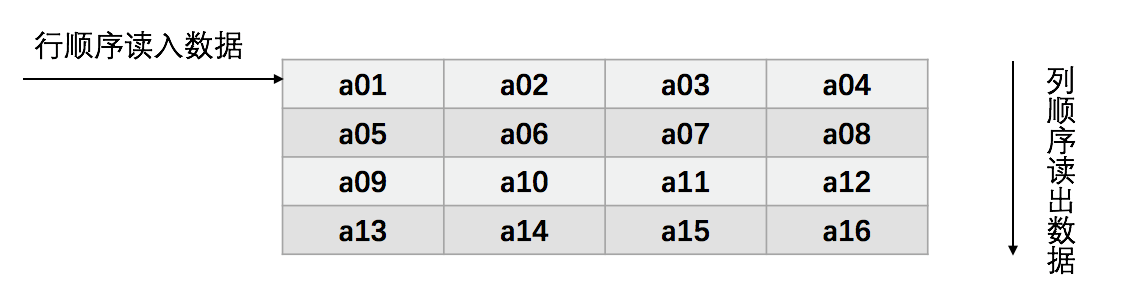
\includegraphics[width=\textwidth]{images//inter_input.png}
\end{figure}

即行顺序写入寄存器,列顺序读出。上图交织结果为a01,a05,a09,a13,a02,a06,a10,a14,a03,a07,a11,a15,a04,a08,a12,a16

解交织时方法和交织相同。

本实验中实现行列交织的具体算法为:

使用两个寄存器数组,一个的作用为行顺序接收当前输入数据并存储时另一个负责按照列顺序输出数组中存储数据。每周期读入一个比特,每16个周期两数组作用互换。

每一周期读入比特的流程图如下:

\begin{figure}[htd]
    \centering
    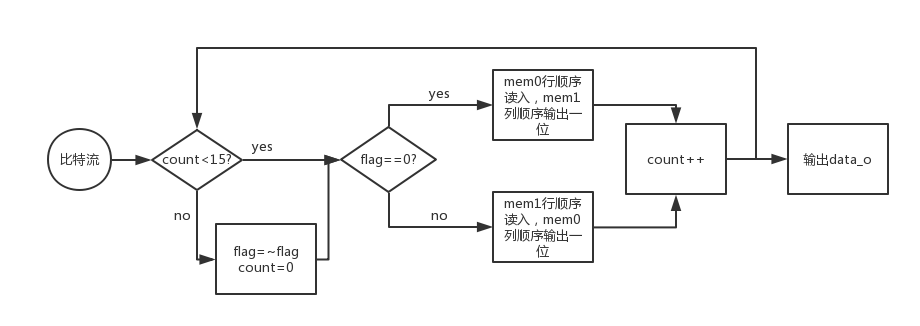
\includegraphics[width=\textwidth]{images//inter_pic.png}
\end{figure}

初始时:count=0;flag=0;mem0[15:0],mem1[15:0]=0;data\_o=0;